% Created 2018-04-13 Fre 14:30
\documentclass[a4paper,ngerman,11pt]{scrartcl}
\usepackage[utf8]{inputenc}
\usepackage[T1]{fontenc}
\usepackage{fixltx2e}
\usepackage{graphicx}
\usepackage{longtable}
\usepackage{float}
\usepackage{wrapfig}
\usepackage{rotating}
\usepackage[normalem]{ulem}
\usepackage{amsmath}
\usepackage{textcomp}
\usepackage{marvosym}
\usepackage{wasysym}
\usepackage{amssymb}
\tolerance=1000
\usepackage{natbib}
\usepackage[linktocpage,pdfstartview=FitH,colorlinks,linkcolor=black,
anchorcolor=black,citecolor=black,filecolor=black,menucolor=black,urlcolor=black]{hyperref}
\usepackage{ngerman}
\usepackage{url}
\usepackage{breakurl}
\addtokomafont{disposition}{\rmfamily}
\setcounter{secnumdepth}{0}
\author{Christian Sangvik, Gruppe 1}
\date{9. April 2018}
\title{Abgabe Material}
\hypersetup{
  pdfkeywords={},
  pdfsubject={},
  pdfcreator={Emacs 25.3.1 (Org mode 8.2.10)}}
\begin{document}

\maketitle


\section*{Wahrnehmungsspaziergang}
\label{sec-1}

Ich habe den Perimeter der Gruppe 1 vom Waidspital her betreten. Dort fällt es
auf, dass die Bebauung entlang der Tièchenstrasse meist aus kleineren Häusern
in kleinen bis mittelgrossen Parzellen besteht. Alle Häuser haben ihren
eigenen kleinen Garten und eigene kleine Eingänge die von der Tièchenstrasse
herunter zum Grundstück führen. Nach Norden sieht man den Wald
des Käferbergs und Schrebergärten. Hier macht das Quartier eigentlich einen
wenig urbanen Eindruck. Lediglich die Tièchenstrasse selber ist relativ stark
frequentiert, sonst könnte man auch meinen, dass man in einem weit abgelegenen
Teil einer Stadt oder gar auf dem Land ist.

\begin{figure}[H]
\centering
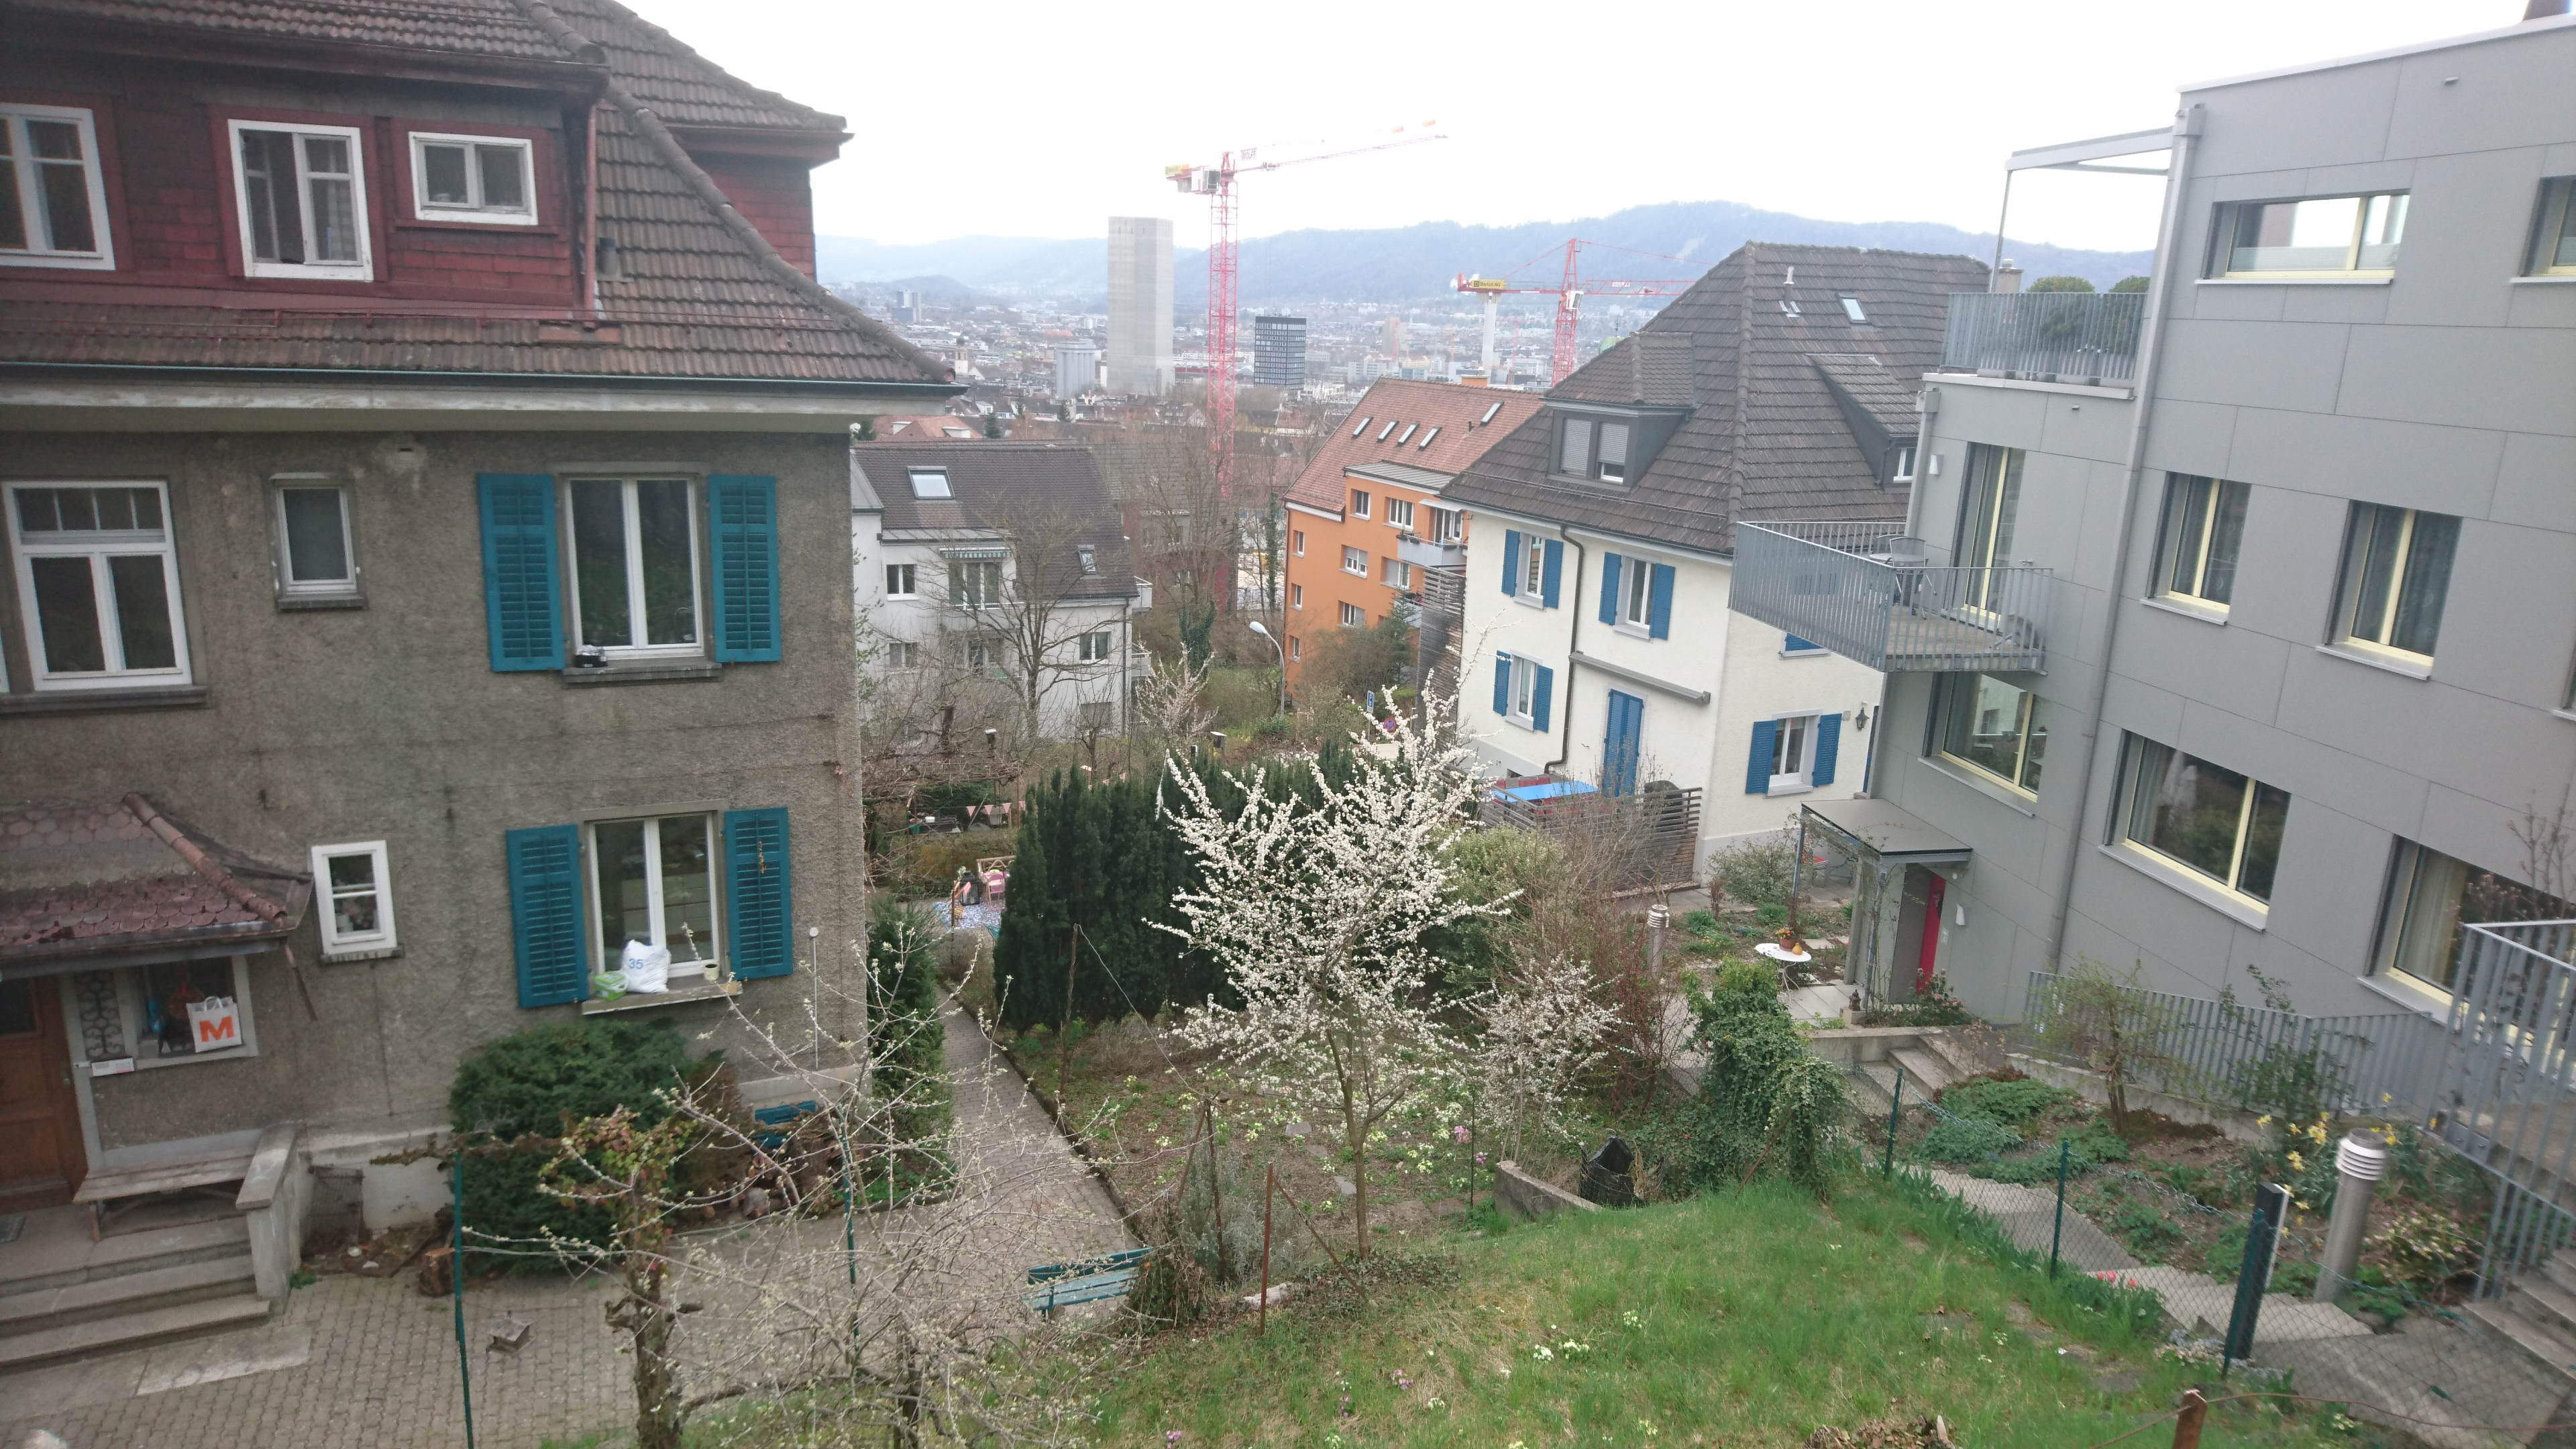
\includegraphics[width=\textwidth]{../Bilder/DSC_0522.JPG}
\caption{Tièchenstrasse, Christian Sangvik, 9.4.18}
\end{figure}

Am Bucheggplatz dann aber zeigt sich aus dem Nichts ein völlig anderes
Bild. Die Bebauung ist viel höher. Der Raum vor mir ist aber trotzdem von der
Horizontalen geprägt. Man sieht überal Asphalt und Verkehrsfläche. Es ist sehr laut
und voller Autos, Lastwagen, Linienbussen und Ampelanlagen. Die Leute hier
bewegen sich hektisch und zielorientiert schnell. Um von einem Punkt zu einem
anderen zu gelangen, der auf der anderen Seite der Strasse ist, muss ich einen
sehr mühsamen Weg über die Fussgängerstreifen wählen, die mit ganz kleinen
Inseln unterbrochen sind und die Ampeln scheinen so geschalten, dass man
überal anhalten muss.

\begin{figure}[H]
\centering
\includegraphics[width=\textwidth]{../Bilder/DSC_0533.JPG}
\caption{Bucheggplatz, Mündung Tièchenstrasse, Christian Sangvik, 9.4.18}
\end{figure}

Die Insel des Bucheggplatzes selber ist gut belebt, allerdings nur von auf den
Anschluss wartenden Pendlern des öffentlichen Verkehres. Nur vor dem neuen
roten Container scheint es ein wenig ruhiger zu sein und die Menschen dort
verweilen an den kleinen Tischen oder auf den Bänken. Die rote Überführung
scheint von Radfahrern und Fussgängern genutzt zu werden, die nicht durch die
Mühseligkeiten des Bodenverkehrs wollen. Alles in allem wirkt der Platz auf
mich aber sehr kalt und abweisend. Es sind viele Menschen hier, doch wenig
Leben.

Weiter in den Perimeter ändert sich dieses Bild kaum. Man sieht im Aussenraum
kaum Menschen, die Bauten wirken sehr introvertiert. Das Prägende am ganzen
Quartier ist aber auf jeden Fall der Verkehr und das Mangeln von verweilenden
Menschen. Angebot für ein Quartierleben gibt es kaum. Ich habe ein
Chinarestaurant gesehen, einen Kiosk, den Denner und den neuen roten
Container. Ansonsten gibt es hier scheinbar nichts, was ein Quartierleben
stützen würde.

\begin{figure}[H]
\centering
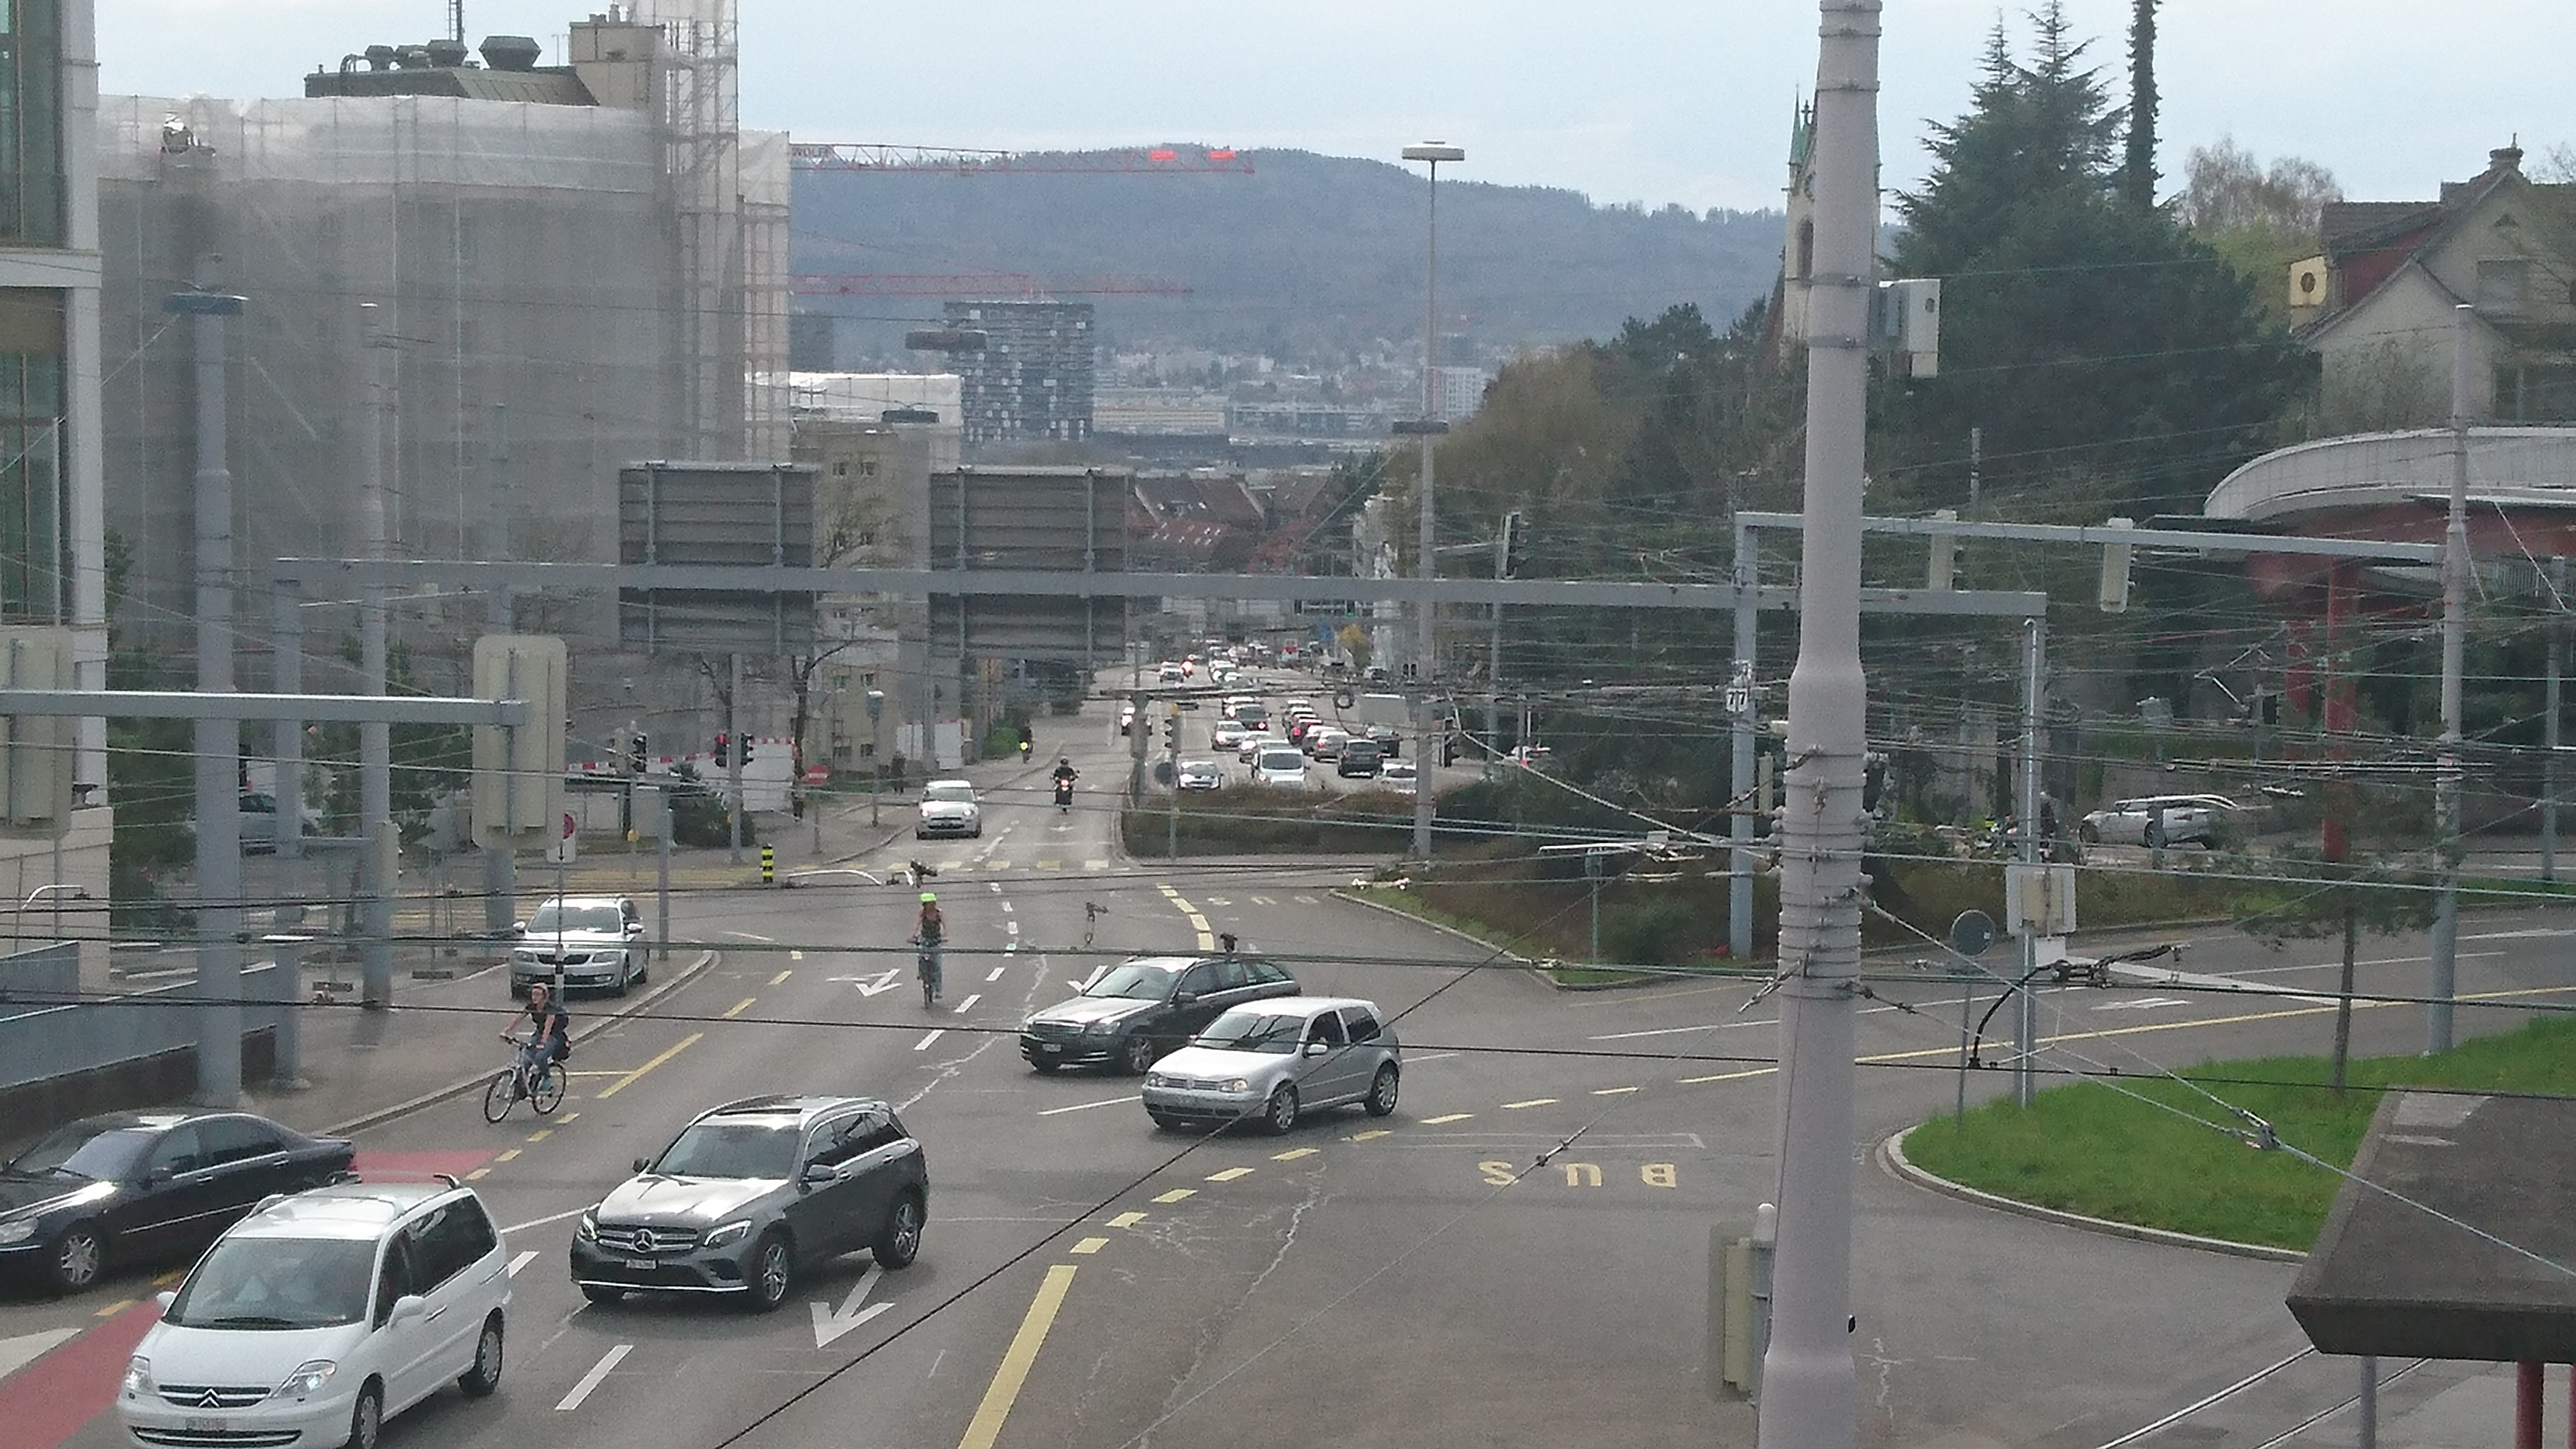
\includegraphics[width=\textwidth]{../Bilder/DSC_0555.JPG}
\caption{Bucheggplatz, Ausblick Rosengartenstr., Christian Sangvik, 9.4.18}
\end{figure}

Ich habe mich persönlich in diesem Quartier nicht sonderlich wohl gefühlt und
war froh es bald wieder verlassen zu können. Schon nach kurzer Zeit hatte ich
Kopfweh von der überreizung meiner Sinneswahrnehmungen vorwiegend durch den
Verkehr.

\section*{Beobachtung}
\label{sec-2}

Für die Beobachtung habe ich mich direkt am Bucheggplatz auf die öffentlichen
roten Liegebänke gesetzt, von wo aus ich einen guten Überblick über den
gesamten Bucheggplatz, die Rötelstrasse und den Eingang der Bucheggstrasse
habe. Ich habe mich für diesen Ort entschieden, da ich nach meinem
Wahrnehmungsspaziergang und auch nach meinen Interviews erfahren habe, dass es
um den Bucheggplatz herum eigentlich gar nichts hat, was ein Treffpunkt sein
könnte ausser einem Chinarestaurant und dem Bucheggplatz selber. Einzig die
Dennerfiliale wäre vielleicht auch noch tauglich gewesen, doch habe ich
erfahren, dass trotz der physischen Nähe die Orientierung nicht Richtung
Rosengartenstrasse und Wipkingen, sondern nach Örlikon hin geht.

Der Bucheggplatz ist eine Strassenkreuzung und wird vorwiegend auch so
benutzt. Ich habe zwar die Fahrzeuge nicht gezählt, doch der Lärm und die
schiere Anzahl der Fahrzeuge, die sich in den anderthalb bis zwei Stunden als
ich meine Beobachtungen gemacht habe, waren überwältigend. Trotzdem, dass die
Kreuzung von sehr viel Verkehr geplagt ist und so kaum Platz für das einzelne
Fahrzeug bleibt, habe ich gemerkt, wie agressiv die einzelnen Chauffeure der
Fahrzeuge gefahren sind. Es wurde gehupt und mit aufheuldendem Motor
beschleunigt und zweimal wurden verschiedene Fahrzeuge auch geblitzt.

Der Bucheggplatz scheint auch ein wichtiger Knotenpunkt im öffentlichen
Verkehr zu sein, denn aus jedem Bus oder Tram abgesehen von jenem der Linie 15
stiegen immer sehr viele Leute aus und ein. Durchschnittlich schätze ich aber
den Aufenthalt der meisten Passanten auf fünf Minuten und weniger. Es scheint
niemand ein gesteigertes Interesse daran zu haben dort zu verweilen. Auch die
Zahl der Fusspassanten war sehr gering. Einige Mütter schoben Ihren
Kinderwagen über den Bucheggplatz in Richtung des Gemeinschaftszentrums.

Richtiger gesellschaftlicher Austausch fand aber nur hier am Container statt,
wo die Leute gerne miteinander redeten oder auch mit der Besitzerin des
Containers sich austauschten. Ein Gast sass sogar nieder um ein Buch zu lesen
und erst nach etwa 40 Minuten wieder zu gehen.

\section*{Interview 1}
\label{sec-3}

Mitbesitzerin des Roten Containers am Bucheggplatz

\begin{itemize}
\item Wie lange führen Sie ihr Geschäft hier schon?

Am 5. Dezember eröffnet. Vorher war nichts hier. Wir haben lange daran
gearbeitet unseren Kaffeecontainer zu verwirklichen. Bau- und
Planungseingaben seit 2015.

\item Warum haben Sie diesen Standort gewählt?

Wohnen alle in der Nähe in einer Genossenschaftswohnung. Seit 8 Jahren, die
anderen seit 15 und 20 Jahren. Hat sonst nichts ausser Kiosk und
Dennerfiliale. Wollten Ort, wo man sich treffen kann und Kaffee trinken. Aus
unserer eigenen Not und dem eigenen Wunsch, so einen Ort zu haben, heraus
haben wir gedacht, wenn es sonst niemand macht, dann eröffnen wir einen
solchen Ort. Mit dem Container konnten wir den Platz auch ein wenig von der
lauten Strasse abschirmen. Die roten Bänke hier werden nun auch benutzt was
sie vorher nie wurden auch wenn sie schon lange da standen.

\item Wären Sie gerne an einem anderen Standort, wenn Sie die Möglichkeit hätten?

Dies ist im Moment überhaupt kein Thema.

\item Nutzen Sie das Quartier auch in der Freizeit? Wohnen Sie in der Nähe?

Ja. Wir haben alle Kinder und nutzen das GZ nebenan mit den Tieren und
Spielplatz. Wohnen hier und arbeiten alle in der Umgebung. Sind immer hier
unterwegs.

\item Wie würden Sie ihre Kundschaft beschreiben?

Sehr sehr durchmischt. Wir haben Studenten die hier auf den Bus gehen, um an
die ETH oder Uni Irchel zu gelangen. Aber auch sehr viele Quartierbewohner
wie wir es sind und auch ältere Leute die hierher kommen um einen Kaffee zu
trinken. Wir haben also ein sehr durchmischtes Klientel und das finden wir
auch gut so, dass wir nicht nur eine kleine Gruppe bedienen.

\item Schätzen die Leute hier Ihr Angebot?

Ja sehr. Wir bekommen viel gute Rückmeldung. Der Platz ist ein bisschen mehr
belebt, und das Geschäft läuft sehr gut. Der Start in den Wintermonaten war
ein wenig schwierig weil es auch kalt war und wir nur ein Take-away anbieten
dürfen. Im Frühling jetzt haben wir aber das Gefühl es kommt super. Leider
dürfen wir aber nicht frisch kochen oder grillen, da wir nur eine
aufwärmküche haben dürfen, und für uns die Auflagen für eine ordentliche
Küche nicht tragbar wären.

\item Wie hat sich das Quartier in den letzten Jahren verändert?

Das ist schwierig zum sagen. Es hat viel günstigen Wohnraum. Ich würde es
sehr durchmischt beschreiben, wie unsere Kundschaft. Ein paar neue Häuser
sind entstanden, dort hat sich bestimmt der Mieterspiegel auch
verjüngt. Auch in unserer Genossenschaft scheint dies der Fall zu sein, dass
es vorher noch nicht so viele Junge Leute hatte. Die Kinder können machen
und tun, wie sie wollen und das ist für alle klar und ok. Aber wir haben
dennoch noch viele ältere Leute hier.

\item Wie schätzen Sie die zukünftige Entwicklung für das Gewerbe im Quartier ein?

Wir hoffen, dass das Geschäft gut laufen wird, und haben nicht sonderlich
Angst. Aber wir können halt auch nicht vorhersagen wie es wird. Die Stadt
hat aber geplant die anliegende Brache zu überbauen und es wurden
Eigentumswohnungen erstellt und ich denke dass wir weiter Bestand haben
werden.

\item Finden Sie die Mietpreise angemessen?

Wir wurden ein wenig speziell eingeschätzt, da wir nicht in der Bauzone
sind, und die Stadt selber ein wenig improvisieren musste beim Rahmenwerk
für unseren Container. Der Container gilt als Provisorium und wir bezahlen
Miete, wie wenn wir in einem Aussenquartier wären. Ob die Einschätzung so
bleibt wissen wir nicht. Die Stadt wollte sich offenhalten die Entwicklung
vorzu anzupassen, je nachdem wie dies nun kommt mit der Rosengartenstrasse.
\end{itemize}


\section*{Interview 2}
\label{sec-4}

Passantin am Bucheggplatz in Richtung Rötelstrasse.

\begin{itemize}
\item Sind Sie oft in diesem Quartier unterwegs?

Ja, ich wohne hier, und arbeite ganz in der Nähe. Mit den Kindern gehen wir
oft ins Gemeinschaftszentrum.

\item Wie würden Sie das Quartier beschreiben?

Das Quartier ist sehr laut und es ist gezeichnet von den vielen Autos. Aber
die Leute hier sind freundlich und wir versuchen das beste aus der Situation
zu machen und mit Freude durchs Leben zu gehen.

\item Wie empfinden Sie diesen Ort?

Wie gesagt, ich finde es sehr laut hier, aber trotzdem bin ich eigentlich
immer gerne hier. Ich wohne seit 17 Jahren in einer der
Genossenschaftswohnungen und habe vor allem mit den anderen Menschen die
hier wohnen immer gute Erfahrungen gemacht. Wenn die Strasse weg wäre wäre
dieser Ort für mich perfekt.

\item Was ist Ihr Bezug zum Quartier?

Praktisch mein gesamtes soziales Umfeld ist hier. Meine Eltern wohnen zwei
Häuser weiter, und ich bin jeden Tag hier unterwegs wenn ich zur Arbeit
gehe. Wenn wir etwas brauchen, was es hier nicht gibt, nehme ich das Tram
nach Örlikon und bin schnell da und auch wieder zurück.

\item Wo halten Sie sich im Quartier auf?

In unserer Genossenschaftssiedlung treffen wir uns häufig im Hof und
sprechen miteinander, wenn ich einkaufen muss, dann gehe ich für das meiste
in den Denner, sonst sind wir noch oft im Gemeinschaftszentrum oder gehen
Richtung Wald oder Schrebergärten, die sehr nahe sind.

\item Wie finden Sie die Wohnqualität hier?

Die Wohnqualität selber ist eigentlich recht gut. Wir sind sehr zentral
hier, sind aber in kurzer Zeit an einem ganz ruhigen Ort. Die öffentliche
Erschliessung ist super, es ist eigentlich nur der Verkehr der viel zu laut
ist.

\item Wie hat sich das Quartier in den letzten Jahren verändert?

Nicht gross. Es gibt ein paar neue Häuser und weiter unten entlang der
Rosengartenstrasse wird viel gebaut. Aber hier am Bucheggplatz ist abgesehen
von diesen neuen Gebäuden nicht viel anders geworden. Wenn es so kommt, wie
ich es ehrlichgesagt auch hoffe, dass der Privatverkehr durch den Tunnel
geführt wird wird es nochmal ein wenig ruhiger und können an der
Rosengartenstrasse dann auch massiv teurere Preise auffahren. Aber hier um
den Bucheggplatz sind so viele Genossenschaftsbauten, wo wir weiterhin
günstig wohnen können.

\item Finden Sie ihre Miete angemessen?

Meine Miete in der Genossenschaft ist sehr angemessen. Aber ich habe auch
eine Neubauwohnung einer Genossenschaft gesehen, die auch völlig in Ordnung
ist.

\item Wenn Sie könnten, was würden Sie im Quartier verändern?

Ich würde die laute Strasse wegmachen (lachend).

\item Welchen Einfluss hat die Rosengartenstrasse auf das Quartier und Ihr Leben?

Auf den Bucheggplatz hat die Strasse vor allem den Einfluss dass es sehr
laut ist und sehr ungemütlich. Nicht prinzipiell wegen dem öffentlichen
Verkehr sondern schon vor Allem wegen dem Privatverkehr. Der meiste Verkehr
ist kein Zubringer, sondern nur Durchgangsverkehr. Wir hatten

\item Gefällt es Ihnen hier zu wohnen?

Ja eigentlich sehr. Das Quartier hat viel zu bieten, abgesehen davon dass es
laut ist. Man ist in sehr kurzer Zeit im Wald und wir haben einen
Schrebergarten im Waid. Ausserdem ist das GZ super und das Bad Allenmoos ist
nur zwei Tramstationen entfernt. Wir orientieren uns mehr Richtung Örlikon
als in Richtung Stadt. Ich wüsste nicht, warum ich in das Chaos hinunter
sollte.

\item Ist der Bezug nach Wipkingen stark?

Wir hatten unsere Kinder in der Krippe in Wipkingen und sind daher doch oft
hergekommen. Ich hatte aber jedes mal Mitleid mit denjenigen die an der
Rosengartenstrasse leben müssen. Dies sind ja meist die gesellschaftlich
schwächer gestellten. Dies wird sich aber sicherlich ändern, wenn die
Strasse beruhigt wird.
\end{itemize}
% Emacs 25.3.1 (Org mode 8.2.10)
\end{document}
